%\documentclass[pdftex,dvipsnames,usenames,aps,superscriptaddress,twocolumn,amsmath,showkeys]{revtex4-1}
\documentclass[pdftex,dvipsnames,usenames,fleqn,12pt]{article}

\usepackage{hyperref}
\usepackage{float}
\usepackage{dcolumn}
\usepackage{graphicx}
\usepackage{color}
\usepackage{amssymb}
\usepackage{bold-extra}
\usepackage{caption}
\usepackage{subcaption}
\usepackage{verbatim}

\usepackage{lineno}
%\usepackage{lineno, blindtext}
%\begin{document}
%    \blindtext
%    \begin{linenumbers}
%        \blindtext
%    \end{linenumbers}
%Some text.\linelabel{lne:label1}
%    \clearpage
%    See line \lineref{lne:label1}.


%\usepackage{cuted} % to generate 1 column text via \begin{strip}    \lipsum[3-4]    \end{strip}

%\usepackage{subfigure}

%%%%%%%%%%%%%%%%%%%%
%  Load shortcut definitions of journals
\input{C:/OlafsUtil/LocalTex/Preambule-Refs}
%\input{Preambule-Refs}
%%%%%%%%%%%%%%%%%%%%%%%%%%%%%
\newcolumntype{d}[1]{D{.}{.}{#1} }
\newcolumntype{h}[1]{D{-}{-}{#1} }

\oddsidemargin -.7cm
%\evensidemargin .5cm
\textwidth 17cm

\def\vB{{\bf{v}\times\bf{B}}}
\def\vvB{{\bf{v}\times\left(\bf{v}\times\bf{B}\right)}}

\hyphenation{e-va-po-ra-tion}
\def\beq{\begin{equation}}
\def\eeq{\end{equation} }
\def\bea{\begin{eqnarray}}
\def\eea{\end{eqnarray}}
\def\lbar#1{\overline{#1}}

%\def\prog#1{\mbox{\bf #1}}

\def\appref#1{Appendix~\ref{app:#1}}
\def\applab#1{\label{app:#1}}  % Put in caption
\def\figref#1{Fig.~\ref{fig:#1}}
\def\figlab#1{\label{fig:#1}}  % Put in caption
\def\eqref#1{Eq.~(\ref{eq:#1})}
\def\eqsref#1#2{Eqs.~(\ref{eq:#1},\ref{eq:#2})}
\def\eqlab#1{\label{eq:#1}}
\def\tabref#1{Table~\ref{tab:#1}}
\def\tablab#1{\label{tab:#1}}  % Put in caption
\newcommand*{\secref}[1]{Section~\ref{sec:#1}}
\newcommand*{\seclab}[1]{\label{sec:#1}}
\newcommand{\Omit}[1]{}
\newcommand{\Olaf}{\color[named]{Purple}}
\newcommand{\RED}{\color[named]{Red}}
\newcommand{\BLUE}{\color[named]{Blue}}
\newcommand{\Stijn}[1]{{\marginpar{\RED Stijn}\RED\bf #1}}
\newcommand{\Krijn}[1]{{\marginpar{\BLUE Krijn}\BLUE\bf #1}}
\newcommand{\os}[1]{{\marginpar{\Olaf Olaf}\Olaf\bf #1}}
\newcommand{\OS}[2]{{\color[named]{Green}\small {\it old:} #1}{\Olaf {\it new:} \bf #2}}
\newcommand{\m}[1]{{\marginpar{\RED\textbullet}\RED #1}}
\newcommand{\mm}[1]{{\RED \textbullet #1 \textbullet}}
\def\Xmax{X_{\rm max}}
\def\Xrh{X_{\rm z}}
\def\Prog#1{ & = {\tt #1} }
\def\SName{MGMR3D}
\newcommand{\Added}[2]{{\marginpar{\RED \bf #1}\RED\bf #2}}

\newcommand{\uvect}[1]{\mathbf{\hat{#1}}}
\def\KVI{University of Groningen, KVI Center for Advanced Radiation Technology, Groningen, The Netherlands}
\def\AIVUB{Astrophysical Institute, Vrije Universiteit Brussel, Pleinlaan 2, 1050 Brussels, Belgium}
\def\VUB{Vrije Universiteit Brussel, Dienst ELEM, Brussels, Belgium}
\def\NIKHEF{Nikhef, Science Park Amsterdam, Amsterdam, The Netherlands}
\def\IMAPP{Department of Astrophysics/IMAPP, Radboud University Nijmegen, Nijmegen, The Netherlands}
\def\CWI{CWI, Centrum Wiskunde \& Informatica, Amsterdam, The Netherlands}
\def\TUe{TU/e, Eindhoven University of Technology, Eindhoven, The Netherlands}
\def\ASTRON{Netherlands Institute for Radio Astronomy (ASTRON), Dwingeloo, The Netherlands}
\def\MPIB{Max-Planck-Institut f\"{u}r Radioastronomie,  Bonn, Germany}
\def\UCI{Physics and Astronomy, University of California, Irvine, CA 92697-4575,U.S.A}

\begin{document}

\begin{centering}
{\LARGE  \bf \textsc{mgmr3d\_fit}; The guide}

{\Large Olaf Scholten}

 {scholten@kvi.nl}

 \today
\end{centering}

\tableofcontents

\section{Purpose}

{\bf MGMR3D:} Quick calculation of radio footprint to allow fitting. This is implemented as a subroutine called in MGMR3D\_fit.

\bigskip
\noindent{\bf MGMR3D\_fit:} fit a given radio footprint with a model for the structure of the electric fields in the atmosphere.

\section{Used parametrization}

\subsection{atmosphere}

For parameterizing the atmosphere it is important to distinguish $z$, the distance to ground along shower axis, and $H=z\cos{\theta_s}$, the vertical height above ground for an inclined shower at an angle $\theta_s$, ignoring the curvature of Earth. The height dependence of the atmospheric penetration depth is taken as
\beq
\Xrh(z)= \left( a+b\, e^{-H/c} \right) /\cos{\theta_s} \;,
\eqlab{Def-Xrh}
\eeq
where $H$ denotes the height above ground and where the constants $a,b,c$ depend on height as given in \tabref{Atmosphere} for the U.S. standard atmosphere which are the same as used in CORSIKA~\cite{CORSIKA}.

\begin{table}[!ht]
\caption{Parameters used for the air-density profile\tablab{Atmosphere}}
\begin{tabular}{h{3}||d{7}|d{5}|d{5}|}
%h [km] & \multicolumn{1}{c||}{a} & \multicolumn{1}{c}{a} & \multicolumn{1}{c}{a} \\
\hline
\multicolumn{1}{c||}{$H$ [km]} & \multicolumn{1}{c|}{a [g/cm$^2$]} & \multicolumn{1}{c|}{b [g/cm$^2$]} & \multicolumn{1}{c|}{c [m]} \\
\hline
10-20 & 0.61289 & 1305.5948 & 6361.4304\\
4-10  & -94.919 &  1144.9069 &  8781.5355 \\
0-4  & -186.555305 &  1222.6562 &  9941.8638\\
\hline
\end{tabular}
\end{table}

The dependence of the index of refraction on the height in the atmosphere is taken as given by the Gladstone�-Dale relation,
\beq
n_{GD}=1+n_\rho \rho(z) \;, \eqlab{GD}
\eeq
where $n_\rho$ is the refractivity at ground level.

\subsection{plasma cloud}
The currents (see the MGMR3D~\cite{MGMR3D} for a more detailed description and argumentation) are parametrized as
\beq
j^\mu(t_s,x_s,y_s,h)={w(r_s) \over r_s} \, f(h,r_s) \, J^\mu(t_s) \;.
\eqlab{DefCloud}
\eeq
where -in principle- the parametrization of the plasma cloud can be chosen differently for the transverse current and charge excess, but where in practise they have been taken the same.

The lateral distribution of the plasma cloud is taken as
\beq
w(r_s)=N_w\,\xi (\xi+1)^{-2.5} \;,
\eqlab{Def-w}
\eeq
with $\xi=r_s/M_0$, introducing the Moliere radius $M_0$ as a scaling factor and where $N_w$ is chosen such that $\int w(r)\, dr=1$.

For the current density at a distance $h$ behind the shower front (pancake function) four different parameterizations, selected by {\tt SelectFh}, are implemented
\bea
{\tt SelectFh=1} &\quad& f(h,r_s)=N_f\, \eta^{\alpha} e^{-2\eta} \;, \\ % fh=x^alpha e^(-2x), case 1
{\tt SelectFh=2} &\quad& f(h,r_s)=N_f\, {\eta \over e^{\eta} + 1 } \;, \\ % fh=x /(exp(sqrt(x))+1), case 2
{\tt SelectFh=3} &\quad& f(h,r_s)=N_f\, {\eta^{2} \over e^{\sqrt{\eta}} + \alpha } \;, \\ % fh=x^2 /(exp(sqrt(x))+c*alpha), case 3
{\tt SelectFh=4} &\quad& f(h,r_s)=N_f\, {\eta \over e^{\sqrt{\eta}} + 1}\;,  % case 4
\eqlab{Def-f}
\eea
where $\eta={h/ \lambda}$.  The norm, $N_f$ is chosen such that $\int_0^\infty f(h,r_s) dh=1$ for all values of $r_s$.
The pancake-thickness scaling parameter
\beq
\lambda(r_s,|F|)= \Lambda(r_s) \, \alpha(|F|) \;,
\eqlab{Def-lam}
\eeq
is factorized in a dependence on distance to the shower axis, $r_s$,
\beq
\Lambda(r_s)= \max[\Lambda_0, \Lambda_1 {r_s\over r_1} ] \quad \;,
\eqlab{Def-lamr}
\eeq
and a scale parameter $\alpha(|F_\perp|)$ that depends on the net transverse force, see \eqref{FE}, acting on the particles in the plasma cloud,
\beq
\alpha(|F_\perp|)= 1 + a_0 \, \sqrt{\Xrh/\Xmax}
                    + a_E \, \left| {\vec{F}_\perp \over 100\, {\rm [keV/m]}} \right|^2 \;.
\eqlab{Def-alphaE}
\eeq

\subsection{longitudinal profile}

The number of charged particles is written as
\beq
N_{c}(\Xrh)= \left({ \Xrh-X_0 \over \Xmax -X_0}\right)^{(\Xmax -X_0)/ \gamma} e^{(\Xmax - \Xrh)/\gamma}
\eqlab{Def-Nc}
\eeq
where $\gamma$ is a parameter controlling the width of the distribution and $X_0$ the point of initial interaction.

The transverse current, see \eqref{DefCloud}, is obtained by multiplying the number of charged particles with the drift velocity,
\beq
\vec{J}_\perp(t_s)= N_{c}(\Xrh) \,\vec{u}_\perp(\Xrh)
\eqlab{Def-It}
\eeq
where the induced transverse drift velocity is denoted as $\vec{u}_\perp$.
\beq
\vec{u}_\perp(\Xrh)=c \vec{\upsilon} /\sqrt{1 +\upsilon^2/\upsilon_0^2} \;,
\eqlab{Def-u}
\eeq
where the parameter $\upsilon_0$, as discussed later, is taken such that for fair weather conditions one is still in the regime where the drift velocity scales linearly with the Lorentz force. When not too large, the drift velocity is proportional to the force acting on the plasma charges,
\beq
\vec{\upsilon}(\Xrh)= {\vec{F}_\perp \over F_\beta}\, {(1+a_t)^2\Xrh\, \sqrt{\Xmax\,X_v}\over (\Xmax + a_t\,\Xrh)^2 } \;,
\eqlab{Def-sigma}
\eeq
where $F_\beta$ represents a friction constant, $a_t=2$ (hard coded in {\tt Subroutine Initialize\_shower}, and a normalization constant of $X_v=500$~g/cm$^2$ is used in the MGMR3D paper. This does not work for horizontal showers and is therefore superseded by the more simple
\Added{22/07/'18}{Replaced parametrization that also works for horizontal showers:}
\beq
\vec{\upsilon}(\Xrh)= {\vec{F}_\perp \over F_\beta}\, %{(1+a_t)\,X_v \over (X_v + a_t\,\Xrh) },  \quad (a_t=1)
{1+a_t \over (\Xmax-X_0)/(\Xrh-X_0) + a_t}\,{0.06 \over \rho(z)} \;,
\eqlab{Def-sigma-1}
\eeq
with $\rho(z)$ [g/cm$^2$/m] as the air density and $a_t=3$. Results are shown in \figref{v-drift} for GRAND
(\verb<J0T = 16.8, zen_B=27. , azi_B=-90. <) and with \verb<F_OVER_BETA=  250.0<.

\begin{figure}[ht]
    \centering
    \begin{subfigure}[b]{0.3\textwidth}
        \includegraphics[width=\textwidth]{TC-tr.pdf}
        \caption{Vertical shower with $X_0$=180 and $\Xmax$=820}\figlab{v-drift-vert}
    \end{subfigure}
    ~ %add desired spacing between images, e. g. ~, \quad, \qquad, \hfill etc.
      %(or a blank line to force the subfigure onto a new line)
    \begin{subfigure}[b]{0.3\textwidth}
        \includegraphics[width=\textwidth]{TC-tr-H.pdf}
        \caption{Horizontal shower at various heights} \figlab{v-drift-hor-rho}
    \end{subfigure}
    \begin{subfigure}[b]{0.3\textwidth}
        \includegraphics[width=\textwidth]{TC-H3000-X.pdf}
        \caption{Horizontal shower at various energies} \figlab{v-drift-hor-Xmax}
    \end{subfigure}
\caption{\small
CONEX-MC results for the drift velocity are compared with the parametrization of \eqref{Def-sigma-1}. The GRAND magnetic field is used.}\figlab{v-drift}
\end{figure}

%Lorentz force is acting, $\vec{F}_\perp=e \vec{v}_s \times \vec{B}$

The longitudinal current due to charge excess is defined as,
\beq
J_Q(z)=N_{c}(\Xrh)  \, \rho_c(\Xrh) \;,
\eqlab{Def-IQ}
\eeq
where,
\beq
\rho_c(\Xrh)=J^0_Q\,{1+a_c \over a_c+ \Xmax/\Xrh} \;,
\eqlab{Def-rhc-old}
\eeq
with $a_c=A\_CHX= 0.5$
\Added{22/07/'18}{Replaced parametrization that also works for horizontal showers:}
\beq
\rho_c(\Xrh)=J^0_Q\,
\left( {\Xrh - \Xmax \over (Xmax_0 + \Xrh - X_0)\, a_c} +1 \right) \left( 1 - e^{-5{\Xrh - X_0 \over \Xmax - X_0}} \right)\;,
%    b=(X_rh-X_max)/(Xmax_0+X_rh-X_0)
%   IQ(i)=J0Q* NPart*  ((b/a_ChX) +1.) * (1.d0-exp(-5.d0*((X_rh-X_0)/(X_max-X_0))))
\eqlab{Def-rhc}
\eeq
 with $a_c=A\_CHX$, $J^0_Q=J0Q$  and \verb<A_CHX= 2.5 , J0Q = 0.25 < and $Xmax\_0 = 500$ (hard coded)
models the dependence of the charge excess fraction on penetration depth shown in \figref{ChEx}
%fitted value was J0Q=.25 but apparently the B and V should not have been taken perp but with 27 deg thus F_over_beta should be reduced by a factor 0.89 (=250 not 280)

\begin{figure}[ht]
    \centering
    \begin{subfigure}[b]{0.3\textwidth}
        \includegraphics[width=\textwidth]{CX-tr.pdf}
        \caption{Vertical shower with $X_0$=180 and $\Xmax$=820}\figlab{v-drift-vert}
    \end{subfigure}
    ~ %add desired spacing between images, e. g. ~, \quad, \qquad, \hfill etc.
      %(or a blank line to force the subfigure onto a new line)
    \begin{subfigure}[b]{0.3\textwidth}
        \includegraphics[width=\textwidth]{CX-tr-H.pdf}
        \caption{Horizontal shower at various heights} \figlab{v-drift-hor-rho}
    \end{subfigure}
    \begin{subfigure}[b]{0.3\textwidth}
        \includegraphics[width=\textwidth]{CX-H3000-X.pdf}
        \caption{Horizontal shower at various energies} \figlab{v-drift-hor-Xmax}
    \end{subfigure}
\caption{\small
CONEX-MC results for the charge excess fraction are compared with the parametrization of \eqref{Def-rhc}.}\figlab{ChEx}
\end{figure}

The transverse force is taken as
\beq
\vec{F}_\perp=e \left[ \vec{v} \times \vec{B} + \vec{E}_\perp \right] \;, \eqlab{FE}
\eeq
where $\vec{v} \times \vec{B}=J^0_T \sin \alpha$

\subsection{Moving dipole charge distribution}

Due to the continuity equation we have $d j_x/dx =dQ/dt$, thus for $r_s=\sqrt{x_s^2+y_s^2}$ using $\vec{j}_\perp(t_r,x_s,y_s)=(J_x(t_r) \hat{x} + J_y(t_r) \hat{y} )\, w(r_s)/r_s $ and radial symmetry one can show that
\beq
Q^D(t_r,x_s,y_s)%&=& \left[\int_{-\infty}^{t_r} J_x(t) dt\right] \times  {d\, w(r_s)/r_s \over dx_s} \nonumber \\ &=&
= \int_{-\infty}^{t_r} \! dt \,{\vec{J}_\perp(t)\cdot \vec{r}_s \over r_s}\; {d\, w(r_s)/r_s \over dr_s} \;. \eqlab{QD}
\eeq
Due to the sign change of $\left(\vec{J}_\perp(t)\cdot \vec{r}_s\right)$ at the core, this
corresponds to a dipole charge distribution. This assumes that all particles that were created stay in the shower. In reality they thermalize as was also argued in the previous section.
As a result of this these particles disappear from the shower front, instead they are quasi-static in the atmosphere, and we expect a loss of moving charge proportional to $e^{-X/(\eta X_0)}$. We therefore introduce
\beq
\vec{J}^D(t_r)=\int_{-\infty}^{t_r} \vec{J}(t) \,e^{-[X(t_r)-X(t)]/(\eta X_0)}\,dt \;,
\eqlab{JD}
\eeq
where $X$ depends on $t$ through its dependence on the height in the atmosphere. In \eqref{JD} $X_0$ is the electron mean free path and $\eta$ a parameter that is adjusted to get best agreement with microscopic shower calculations.
The contribution to the radiation field can now be calculated as
\bea
E_x^D &=& -\int dx_s\,dy_s\,{d\, w(r_s)/r_s \over r_s\, dr_s}\, I^D_x\\
 I^D_x &=& \int dh \, f(h) \left. {J^D_x\over n{\cal D}} \right|_{h} \;,
\eea
and a similar expression for $E_y^D$. A small radial polarization component has been neglected at this stage.

\subsubsection{Observables}

In terms of the sampled pulse in the polarization direction $p$, where the complex voltage of the $i^{th}$ sample are denoted as ${\cal E}_{i,p}=E_{i,p} + i\hat{E}_{i,p}$, the Stokes parameters can be expressed as
\begin{eqnarray}
%\\
I&=&{1\over n} \sum_0^{n-1} \left( |{\cal E}|^2_{i,\vB} + |{\cal E}|^2_{i,\vvB} \right) \nonumber\\
Q&=&{1\over n} \sum_0^{n-1} \left( |{\cal E}|^2_{i,\vB} - |{\cal E}|^2_{i,\vvB} \right) \nonumber\\
U +iV&=&{2\over n} \sum_0^{n-1} \left( {\cal E}_{i,\vB} \;  {\cal E}_{i,\vvB}^* \right) \;.
\eqlab{Stokes}
\end{eqnarray}
$\hat{E}_{i,p}$ is the Hilbert transform of the real measured voltage $E_{i,p}$.

\subsubsection{Force-Smoothing}

In order to allow for fitting using a steepest-descent method no fitted shower parameter should change abruptly as function of height since otherwise derivatives cannot be evaluated numerically. For this reason induced transverse current should change smoothly as function of height which is obtained by smoothing the transverse force as function of height. The physics is that from Ref.~\cite{Tri15} we know that after changing the electric field it takes a distance of about 500 [m] before the current is adapted to the new field strength.

Thus the smoothing is applied by multiplying the change in the electric field at an heights $H<h_i$ by a factor
\beq
a=\left[1 + e^{1 + b (H-h_i)}\right]^{-1} \;, \eqlab{Smooth}
\eeq
where
\beq
b=d_{sm} {X(H)-X(H+\delta)\over \delta X_0} \;. \eqlab{D-SM}
\eeq
The parameter value $d_{sm}=2$ is used.

\section{Running MGMR3D}

\subsection{Input}

A typical example of an input is as follows.

\begin{linenumbers}
\begin{verbatim}
  &ShPars IntegrateCurrent=-0.01 , nu_min=0 , nu_max=8000000
   nu_min=30 , nu_max=80
  Intensity_Weight=.false.
 SAMPLINGTIME=5     ! in [ns]
 StParRange = -11    ! in down-sampled sample times for calculation of Stokes parameters
 F_lim=1.
  J0T = 14.77, zen_B=22.19 , azi_B=-90.   ! direction magnetic field at LOFAR (49.5 mu T)
 ! J0T = 16.8, zen_B=27 , azi_B=-90.   ! direction magnetic field at GRAND (56 mu T)
 x_0=200, X_max=690. , GROUNDLEVEL=  0.0
 energy_sh=2.e7, zen_sh=20
  &end

 0.  0.   !  shift_x [m], shift_y [m], alpha_vB [deg]
 step
8.0 51.4198405287 103.495733281
5.0 35.0 -90.0
3.0 21.2132034356 -45.0

 5, 7, 11, 12  0 0
 data\coreas_456_set1_37

grid 25
dist 50
dist 75
dist 250
theta 90.
!-------------------------------------------------------
\end{verbatim}
\end{linenumbers}

\subsubsection{Generic shower parameters}

%\begin{linenumbers}\resetlinenumber
The parameters that specify the general run-parameters of the code and those that specify the structure of the plasma cloud are entered first between the opening \verb< &ShPars < and closing \verb< &end < statements including two parameters that are relevant for fitting. The general format is ``{\tt ParameterName = Value}" separated by commas. All characters entered after the exclamation ``{\tt!}" are treated as comments and will not be processed. When a parameter is not specified it obtains its default value. The list of possible ParameterNames (not case sensitive) is given in \tabref{ShPars}.
%\end{linenumbers}

\begin{table}[!ht]
\caption{Possible {\tt ParameterNames} in the {\tt ShPars} namelist and their default values. \tablab{ShPars}}
\begin{tabular}{|l l |l l|}
\hline
\\  \verb<A_CHX< & = 2.5                  &    \verb<OBSDIST_DIM< & =      42
\\  \verb<ATMHEI_DIM< & =       2000      &    \verb<OBSDIST_STEP< & =  10.0
\\  \verb<ATMHEI_STEP< & =  10.0          &    \verb<PADDING< & =       5000
\\  \verb<F_LIM< & =  1.0                 &    \verb<PANCAKEINCFIELD< & = 0.41
\\  \verb<F_OVER_BETA< & =  250.0         &    \verb<RH0< & =  2.92E-4
\\  \verb<INTEGRATECURRENT< & = -0.01     &    \verb<SAMPLINGTIME< & = 5.0
\\  \verb<INTENSITY_WEIGHT< & =F          &    \verb<SELECTFH< & =       4
\\  \verb<J0T< & =  12.0                  &    \verb<STPARRANGE< & =   11
\\  \verb<J0Q< & = 0.25                   &    \verb<TEST< & =F
\\  \verb<LAM_TC< & =  0.05               &    \verb<TTRACE_STEP< & =  0.02
\\  \verb<LAM_100< & =  7.0               &    \verb<U0< & =  60.0
\\  \verb<LAMX< & =  100.0                &    \verb<X_MAX< & =700
\\  \verb<MOLIERERADIUS< & =  27.0        &    \verb<X_0< & =  36.7
\\  \verb<NU_MIN< & =  30.0               &    \verb<XDEPALPHA< & =  0.0
\\  \verb<NU_MAX< & =  80.0               &    \verb<GroundLevel< & =  0.0
\\  \verb<Zen_sh< & =  0 .0               &    \verb<Azi_sh< & =  0.0
\\  \verb<Zen_B< & =   90.0               &    \verb<Azi_B< & =  0.0
\\  \verb<Energy_sh< & =  1.e9            &    & \\
\hline
\end{tabular}
\end{table}


\begin{itemize}
\item{\verb<A_ChX<}; The parameter $a_c$ in \eqref{Def-rhc}

\item{\verb<AtmHei_Dim<}; The number of grid points in $z$, see \eqref{Def-Xrh}.

\item{\verb<AtmHei_Step<};  The grid-step size in $z$, see \eqref{Def-Xrh}, in units of [m].

\item{\verb<F_Lim<};  The limiting electric-field strength when fitting in units of [100~kV/m].

\item{\verb<F_Over_Beta<}; Equals the friction constant $F_\beta$ in \eqref{Def-sigma} in units of [keV/m].

\item{\verb<IntegrateCurrent<}; When positive this is equal to $\eta$ in \eqref{JD}, corresponding to a damping factor used to integrate the induced current over previous times, needed for the calculation of the moving-dipole contribution to the radiation.
    \\ When negative, the moving-dipole contribution is not included.

\item{\verb<Intensity_Weight<}; If .false., use error bars specified in the data file.
\\ if .true., set error bars on all Stokes parameters equal to 10\% of the intensity.

\item{\verb<J0T<}; Equals $J^0_T=c \vec{B}$ and determines the magnetic field of Earth, see \eqref{FE}, in units [kV/m] ($J^0_T$[kV/m] = c[m/s] * B[T] /1000 = 30 * B[G]).

\item{\verb<J0Q<}; The normalization constant $J^0_Q$ of the charge excess contribution, see \eqref{Def-rhc}.

\item{\verb<Lam_TC<}; Equals $\Lambda_0$ in \eqref{Def-lamr} in units [m].
\item{\verb<Lam_100<}; Equals $\Lambda_1$ in \eqref{Def-lamr} in units [m].

\item{\verb<LamX<}; Equals $\gamma$ in \eqref{Def-Nc} in units of [g/cm$^2$].

\item{\verb<MoliereRadius<}; Equals $M_0$ in \eqref{Def-w} in units of [m].

\item{\verb<Nu_Min<}; Lower edge of the frequency block filter, used in the calculation of observables.
\item{\verb<Nu_Max<}; Upper edge of the frequency block filter, used in the calculation of observables.

\item{\verb<ObsDist_Dim<}; Grid dimension used for the calculation of antenna distance to the shower axis.
\item{\verb<ObsDist_Step<}; Grid spacing used for the calculation of antenna distance to the shower axis, units [m].

\item{\verb<Padding<}; Number of zero-padding added before and after the time traces before down sampling.

\item{\verb<PancakeIncField<}; Equals $a_E$ in \eqref{Def-alphaE}.

\item{\verb<Rh0<}; Refractivity of air at ground level, $n_\rho$ in \eqref{GD}.

\item{\verb<SamplingTime<}; Down-sampling time used for the calculation of observables, in [ns].

\item{\verb<SelectFh<}; Select a particular parametrization for the pancake thickness, see \eqref{Def-f}.

\item{\verb<StParRange<}; Length of time trace in number of down-sampled time-steps (={\tt SamplingTime}) used for calculating observables. If negative the complete trace is used.

\item{\verb<Test<}; If set to .true., additional output is created.

\item{\verb<TTrace_Step<}; Internal sampling time used for the calculations of pulses, in [ns]. Should be rather small for good convergence.

\item{\verb<U0<}; Equals $\upsilon_0 \times F_\beta$ where $\upsilon_0$ is defined in \eqref{Def-u} and $F_\beta$ in \eqref{Def-sigma}, in [kV/m].

%\item{\verb<VDrift2<}; If .true., use \eqref{Def-sigma}, otherwise \eqref{Def-sigma-1}

\item{\verb<X_0<}; Equals $X_0$ in \eqref{Def-Nc} in units of [g/cm$^2$], depth of the first interaction.

\item{\verb<X_max<}; Equals $X_{\rm max}$ in \eqref{Def-Nc} in units of [g/cm$^2$], depth of the shower maximum.

\item{\verb<XDepAlpha<}; Equals $a_0$ in \eqref{Def-alphaE}.

\Added{11/02/'18}{New options:}
\item{\verb<GroundLevel<}; Height above sea level of the shower plane, in [m].
\item{\verb<Zen_sh<}; Zenith angle of the shower, in deg.
\item{\verb<Azi_sh<}; Azimuth angle of the shower, in deg, [East: Azi=0; North: Azi=90]
\\ \Added{15/07/'18}{GRAND option:}
\\if this angle exceeds 70$^\circ$ the program assumes a horizontal shower. The penetration depth at the top-height is set to zero!
\item{\verb<Zen_B<}; Zenith angle for the Earth magnetic field.
\item{\verb<Azi_B<}; Azimuth angle for the Earth magnetic field. If =zero, this is not used for the calculation of the angle between shower and magnetic field.
\item{\verb<Energy_sh<}; Shower energy in [GeV]. Used to set the number of shower particles at the maximum equal to $N_{\rm max}$=\verb<Energy_sh<.
\end{itemize}

\subsubsection{Specific shower parameters}

The line

\begin{linenumbers}\resetlinenumber[12]
\noindent\verb<  0.  0.   !  shift_x [m], shift_y [m], alpha_vB [deg] <;
\end{linenumbers}
The shifts in core position is set to zero [m] relative to the antenna positions entered in the data file;
\\\Added{11/02/'18}{New:}If \verb<Azi_B<=0, the angle $\alpha$ between the Earth magnetic field and the shower axis, see \eqref{FE}, is set to 90$^\circ$. When \verb<Azi_B<$\ne$0 the angle \verb<alpha_vB<=0 is calculated from the specified shower and magnetic field angles.

\bigskip
There are three possible options for specifying the atmospheric electric fields, {\tt\bf step}, {\tt\bf stpv} and {\tt\bf line}. Note that these are case sensitive. If different characters are entered the electric-field nodule is skipped.
\begin{description}
\item[{\tt\bf step};] The following, at most 4 lines, specify height [km] and the change in the electric field (strength [kV/m] and angle [deg]) at this height counted from above. As an additional parameter the value for $d_{sm}$ (see \eqref{D-SM}) can be given, if absent $d_{sm}=2$.
\item[{\tt\bf stpv};] The following, at most 4 lines, specify height [km] and value of the electric field (strength [kV/m] and angle [deg]) in the layer starting at this height. Internally these values are converted to those of the {\tt step} option because these are more stable when fitting. As an additional parameter the value for $d_{sm}$ (see \eqref{D-SM}) can be given, if absent $d_{sm}=2$.
\item[{\tt\bf line};] The following, at most 6 lines, specify height [km] and value of the electric field (strength [kV/m] and angle [deg]) at this height. These values are linearly interpolated for the calculation of the electric field.
\end{description}
The height is height above ground. The input of the atmospheric electric field is terminated by an empty line.

\subsubsection{Fit parameters}\seclab{FitPar}

The lines

\begin{linenumbers}\resetlinenumber[18]
\noindent\verb< 4, 9, 10, 11, 12  0 0<
\\\verb< "data\coreas_456_set1_37" "Results"<
\end{linenumbers}
specify the parameters that should be fitted and the file that contains the data. The entry "Results" is optional.

The first line specifies which parameters can be fitted, where the order of the parameters is:
\\\verb<    J0Q,    lamx,     X_0,   X_max,  lam_tc, lam_100, XDepAlp, MollyRd, Shift_x, Shift_y,<
\\\verb<h_frc-1, h_frc-2, h_frc-3, h_frc-4, Force-1, Force-2, Force-3, Force-4, a_frc-1, a_frc-2,<
\\\verb<a_frc-3, a_frc-4,<
as is also specified in the output of the program. It should be noted that the parameters for the atmospheric electric field depend on the option used ('step', 'stpv', 'line', or 'none'). In this calculation thus the  parameters $\#4=\Xmax$, $\#9=Shift\_x$, $\#10=Shift\_y$, $\#11=h_{frc}1$ (the height associated with the second layer), and $\#12=h_{frc}2$ are fitted.
\\The parameters should be specified in increasing order. The list {\bf terminates} when a lower parameter number is given.
\\{\bf No parameter fitting} will be done when the first parameter number is =0 or negative.

The second line specifies the name of the input file that contains the data to which the present calculation is compared. The intensity is normalized to the intensity in the data and a $\chi^2$ value is calculated. 
\\When a {\bf non-existing file} is specified a straight MGMR3D calculation is performed.
\\It is an option to specify on the same line the name of a file, \verb< "Results"< in the example, to which the {\bf results} for each antenna should be written. If no file is specified the default file \verb<plot/FitResult.dat< is taken
\\\Added{28/10/'18}{New:} When a file is specified, also the time traces for each antenna will be written in separate files.

\subsubsection{Footprint parameters}\seclab{FoPrPar}

The input lines

\begin{linenumbers}\resetlinenumber[21]
\noindent\verb< grid= 25<
\\\verb< dist 50<
\\\verb< dist 75<
\\\verb< theta 90.<
\end{linenumbers}
specify the options for the antenna geometry for which the Stokes parameters will be calculated.
\\As a {\bf default} option the Stokes parameters will be calculated for the antenna positions specified in data file given in the previous input line. The results will be written to \verb<plot/FitResult.dat< unless specified otherwise. There are 3 options, case and space sensitive.
\begin{description}
\item[{\tt\bf grid}] $d$ 'File'; When $d>0$ the emission is calculated for a star-shaped grid with a radial spacing $d$ in [m].
    \\ When $d<0$ the emission is calculated for an rectangular lattice with spacing $d$ in [m].
    \\ The results are written to files 'File'Stokes.csv and 'File'ttrace......csv see \secref{GrOpFi}. The default is 'File'='plot/grid\_'
\item[{\tt\bf dist}] $R$ 'File'; Calculation is done for a ring with diameter $R$ in [m].
    \\ The time-traces and frequency spectra are written to files 'File''tt-'.....csv and 'File''nu-'......csv see \secref{GrOpFi}. The default is 'File'='plot/dist\_'
\item[{\tt\bf theta}] $\phi$ 'File'; Calculation is done along a radial direction $\phi$ [degree] at distance intervals given by the calculation grid as given by \verb<ObsDist_Step<.
    \\ The ratios of Stokes parameters are written to files 'File'.....csv see \secref{GrOpFi}. The default is 'File'='plot/th\_'
\end{description}

\subsubsection{Data-file format}\seclab{DaFiFo}

The header of the data file named in \secref{FitPar} has two lines and is read in free format. The first line as text, integer, text, real ($\theta$), text, real ($\phi$), the second line is treated as comment. As an example:
\\\verb<!GiaId: 456 azimuth= 270.0, zenith= 0.0 <
\\\verb<!x_antenna, y_antenna, St_I, St_Q, St_U, St_V, sigma_I, sigma_Q, sigma_U, sigma_V<
\\The zenith and azimuth angles for this event are taken as ($\theta$, $\phi$) in degrees.
\\The header is followed by a list where each line specifies the ($x, y$) antenna position, the ($I,Q,U,V$) Stokes parameters followed by their errors ($\sigma I,\sigma Q,\sigma U,\sigma V$) in free format.

At reading in it is checked that the antennas lie within the confines of the internal calculation grid as specified by the parameters \verb<ObsDist_Dim< $\times$ \verb<ObsDist_Step<. If an antenna position falls outside this distance a message is send to output like
\\\verb<Antenna lies outside grid   425.00000000000000      >   420.00000000000000 <
\\and is not used for further processing.

\subsection{Output}

A typical output for \verb<Test=.false.< (with outdated parameter values:

{\scriptsize  %\footnotesize
\begin{linenumbers}\resetlinenumber
\noindent\begin{verbatim}
   MGMR3D_fit, run on 30/11/2017 , started at 17:46:50.463 -------------------------
Mesh in height, number=2000, stepsize=10.0[m], max height=20.0[km]
Mesh in distance from core, number= 42, stepsize= 10.0[m]
alpha_vB= 90.0deg, net Lorentz force = (12.00 [keV/m]) x (sin(alpha)=  1.00 ) = 12.00 [keV/m]
&SHPARS
 TEST=F,
 ATMHEI_DIM=       2000,
 ATMHEI_STEP=  10.000000000000000     ,
 RH0=  2.9200000000000000E-004,
 MOLIERERADIUS=  27.000000000000000     ,
 SELECTFH=          4,
 LAM_TC=  5.0000000000000003E-002,
 LAM_100=  7.0000000000000000     ,
 XDEPALPHA=  0.0000000000000000     ,
 INTEGRATECURRENT= -1.0000000000000000E-002,
 PANCAKEINCFIELD= 0.40999999999999998     ,
 OBSDIST_DIM=         42,
 OBSDIST_STEP=  10.000000000000000     ,
 TTRACE_STEP=  2.0000000000000000E-002,
 INTENSITY_WEIGHT=F,
 VDRIFT2=T,
 F_LIM=  1.0000000000000000     ,
 NU_MIN=  30.000000000000000     ,
 NU_MAX=  80.000000000000000     ,
 PADDING=       5000,
 SAMPLINGTIME= 0.50000000000000000     ,
 STPARRANGE=        11,
 J0T=  12.000000000000000     ,
 J0Q= 0.23999999999999999     ,
 X_0=  36.700000000000003     ,
 LAMX=  90.000000000000000     ,
 U0=  60.000000000000000     ,
 F_OVER_BETA=  300.00000000000000     ,
 A_CHX= 0.50000000000000000     ,
 /
possible fit parameters:
    J0Q,     rh0,   a_ChX,    lamx,   X_max,  lam_tc, lam_100, XDepAlp, Shift_x, Shift_y,
h_frc-1, h_frc-2, h_frc-3, Force-1, Force-2, Force-3, a_frc-1, a_frc-2, a_frc-3,
 data read from file=data\coreas_456_set1_37.dat
 !GiaId:         456 azimuth   270.00000000000000      zenith=   0.0000000000000000
 Antenna lies outside grid   425.00000000000000      >   420.00000000000000
 event number=         456  , # antennas=         128 , Zenith angle=   0.0000000000000000

   start Initialize @ 21:18:41. 81 -------------------------
last true basis-grid time= 168.383, last observer time= 201.806[ns]
Refractivity at ground level=   2.920x 10^{-4}, Moliere radius=  27.0[m]
f(h) shape 4 with L=0.05[m], L@100m= 7.00[m] index for X-dependence =0.00
parametrization radial dependence of \lambda; @r=0: 0.05, @r= 1.0m: 0.07, @r= 420.0m:  29.4
 step definition for E-field, Lorentz:   12.000000000000000        0.0000000000000000
 h= 8.000[km], E_step=  51.420[kV/m] @ 103.5[deg] ; h= 8.000[km], E_true=  51.420[kV/m] @ 103.5[deg]
 h= 5.000[km], E_step=  35.000[kV/m] @ -90.0[deg] ; h= 5.000[km], E_true=  19.209[kV/m] @ 128.7[deg]
 h= 3.000[km], E_step=  21.213[kV/m] @ -45.0[deg] ; h= 3.000[km], E_true=   3.000[kV/m] @  -0.0[deg]
 X_max= 660.00, D=  3.660[km], H=  3.660[km], cos_Zen=1.00
 Curr_Xmax= 532.63, D=  5.280[km], H=  5.280[km], Curr_max=0.101, F_max=0.493 x 100 keV/m
   3.0200177807453594E-005  0.10061872080089533
No integrated charge dipole included
Zenith angle=  0.000 degree
\end{verbatim}
\end{linenumbers}}

Most of this will be self explanatory. A distinction is made between the maximum for the number of particles and the current in the shower. The maximum is given by the penetration depth, height above ground ($H$) and distance to the ground ($D$) along the shower axis.

\subsubsection{plot/FitResult.dat}\seclab{OutFiRes}

This output file, see \secref{FitPar} for naming convention, contains the list of calculated Stokes parameters for each antenna position specified in the data file (see \secref{DaFiFo}).
\\Format:
\\Headerline; Labeling of the content of the columns
\\Each following line, real numbers in free format, giving $(d,\phi)$ distance and azimuth angle of the antenna in the shower plane, $I_{data}, I_{MGMR3D}, \sigma_I$ the input value of the intensity, its calculated value and its input error bar. This is followed by the same entries for the $Q, U, V$ Stokes parameters.

\subsubsection{plot/sh\_Current.dat}\seclab{ShCur}

Gives are the properties of the shower as function of height in the atmosphere. The first line labels the various columns.
\begin{description}
\item[c1] {\bf $z$ [km]} The distance to the ground measured along the shower axis.
\item[c2] {\bf $X_z(z)$ [g/cm$^2$]} Penetration depth, measured along the shower axis.
\item[c3] {\bf $n_\rho\,\bar{\rho}(z)$ } Mean refractivity from this height to the ground.
\item[c4] {\bf $J_x(z)$ } Transverse current in the $x$-direction.
\item[c5] {\bf $J_y(z)$ } Transverse current in the $y$-direction.
\item[c6] {\bf $J_Q(z)$ } Charge excess.
\item[c7] {\bf $z$ [g/cm$^3$]} Air density
\item[c8] {\bf $\alpha(z)$ } The depth dependence of the $\alpha$ parameter in the expression for the pancake function.
\item[c9] {\bf $\tilde{F}_x(z)$ [km]} Smoothed net force in the $x$-direction.
\item[c10] {\bf $\tilde{F}_y(z)$ [km]} Smoothed net force in the $y$-direction.
\item[c11] {\bf $|\tilde{F}| $ [keV/m]} Absolute magnitude of the smoothed net force.
\item[c12] {\bf $\phi$ [degree]} Azimuthal direction of the net force.
\end{description}

\subsubsection{Footprint files}\seclab{GrOpFi}

These files are written when the radio-footprint is calculated, see \secref{FoPrPar} for file-prefix naming options. All are comma-separated-values (.csv) files. All values are given in the shower plane.
\begin{description}
\item[plot/grid\_Stokes.csv] Columns give $d$[m], $\phi$, $I$, $Q$, $U$, $V$ for each antenna on the grid.
\item[plot/grid\_ttrace-'d'-'$\phi$'.csv] Columns give $t$ [$\mu$s], $Re(E_x)$, $Im(E_x)$, $Re(E_y)$, $Im(E_y)$ for the antenna on grid-point given by $d$ and $\phi$.
\item[plot/dist\_tt-'d'.csv] Columns give $t$ [ns], $Re(E_x)$, $Re(E_y)$, $Re(E_r)$, $Re(E_x E_r*)$, $Im(E_x E_r*)$ for an antenna at distance $d$ [m].
\item[plot/dist\_nu-'d'.csv] Columns give $\nu$[GHz], $|E_x|$, $|E_y|$, $|E_r|$, for an antenna at distance $d$ [m]. Here $E_r$ denotes the radial component due to charge excess.
\item[plot/th\_'$\phi$'.csv] Columns give $d$ [m], $\phi$, $I$, $Q/I$, $U/I$, $V/I$ for each antenna on the grid at the azimuth angle $\phi$.
\end{description}

\subsection{figures}

The accompanying figures are made using the GLE (see \href{http://www.gle-graphics.org}{http://www.gle-graphics.org/}
for free download) scripts that are included as part of this package. In \figref{sh-current} data from \verb<sh_Current.dat< are used. \figref{pulse-d} uses the data from \verb<dist_nu-....dat< and from \verb<dist_tt-....dat<.

\begin{figure}[ht]
    \centering
    \begin{subfigure}[b]{0.55\textwidth}
        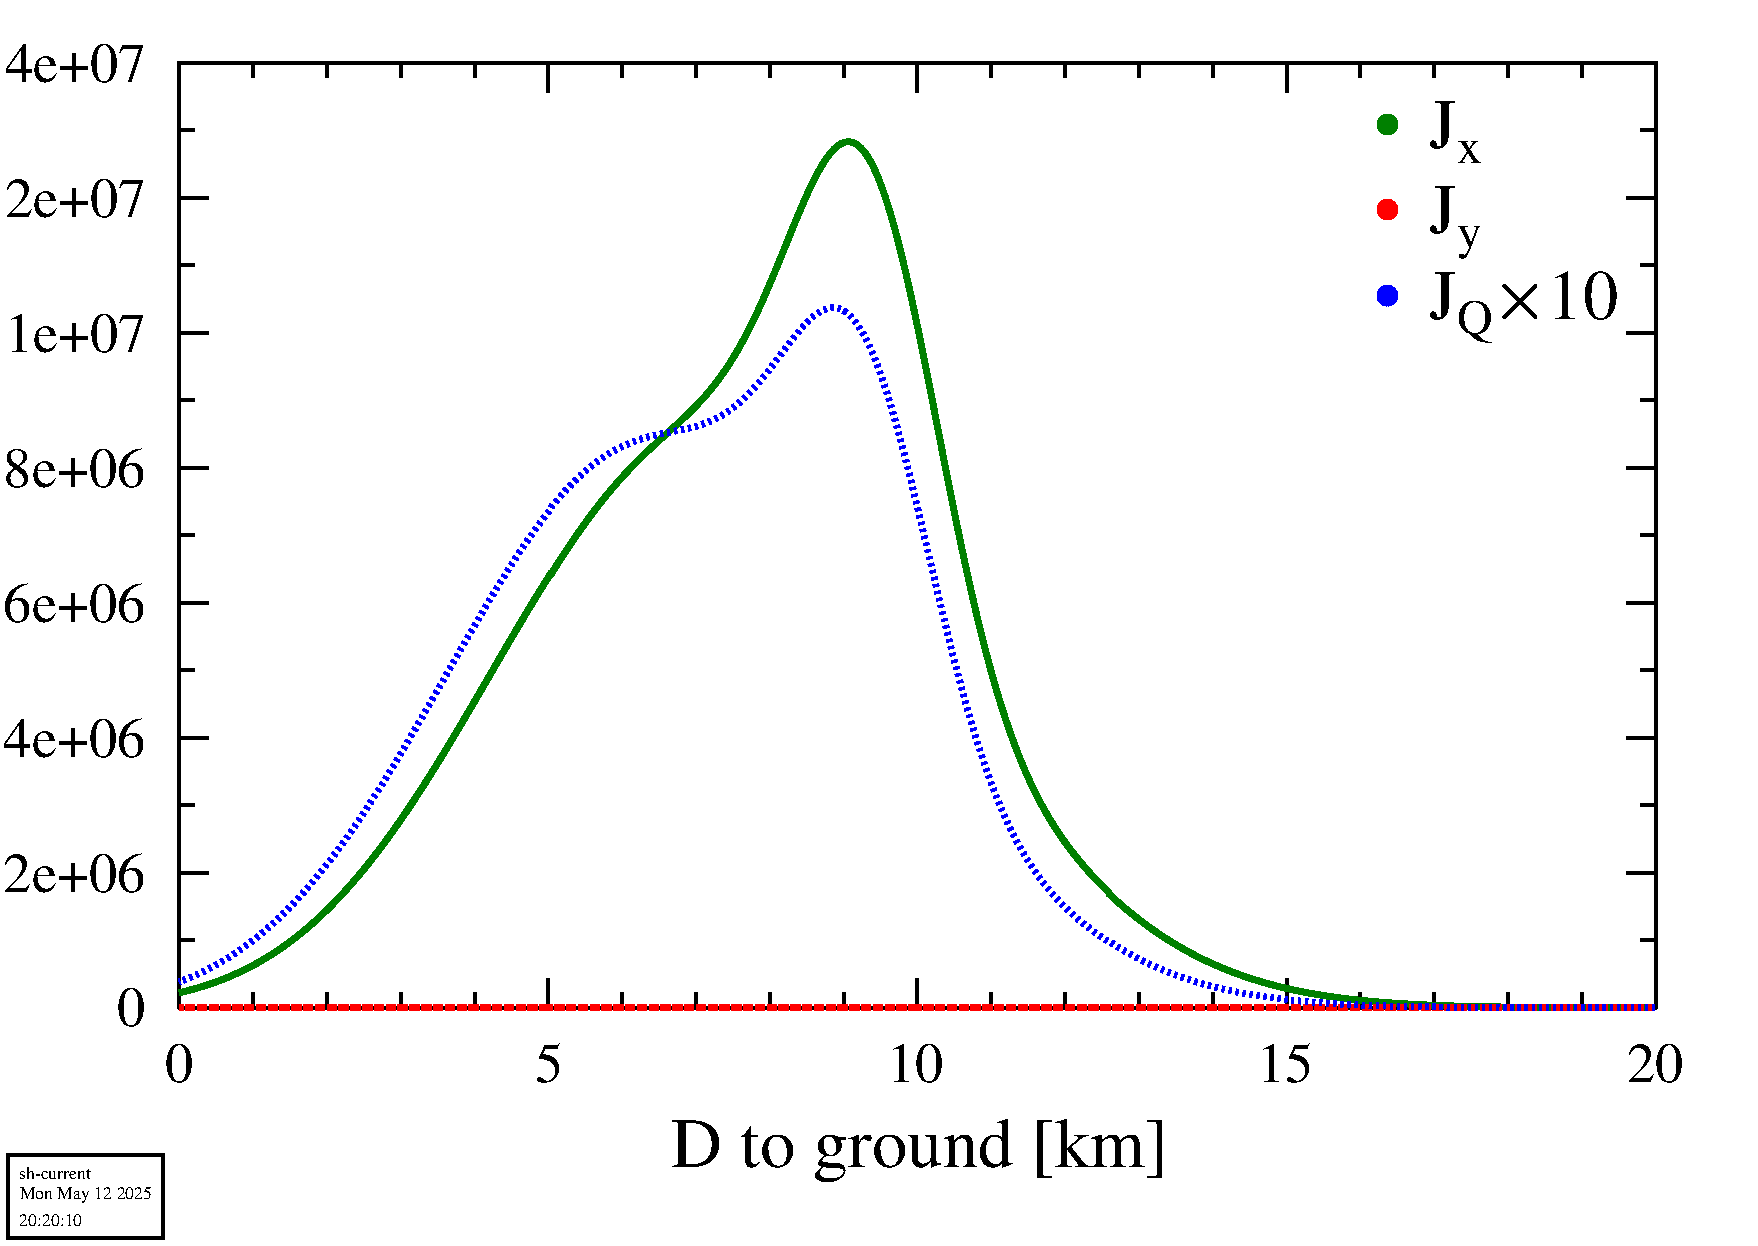
\includegraphics[width=\textwidth]{runs/plot/sh-current.pdf}
        \caption{} \figlab{sh-current}
    \end{subfigure}
    ~ %add desired spacing between images, e. g. ~, \quad, \qquad, \hfill etc.
      %(or a blank line to force the subfigure onto a new line)
    \begin{subfigure}[b]{0.4\textwidth}
        \includegraphics[width=\textwidth]{runs/plot/pulse-d.pdf}
        \caption{} \figlab{pulse-d}
    \end{subfigure}
\caption{\small
Fig.~\subref{fig:sh-current}) shows the currents in the shower plasma as function of distance to Earth, Fig.~\subref{fig:pulse-d}) the pulses in frequency and in time at various distances.  }\figlab{Pulses}
\end{figure}


The Stokes parameters are displayed in \figref{FitStokes}
\begin{figure}[ht]
 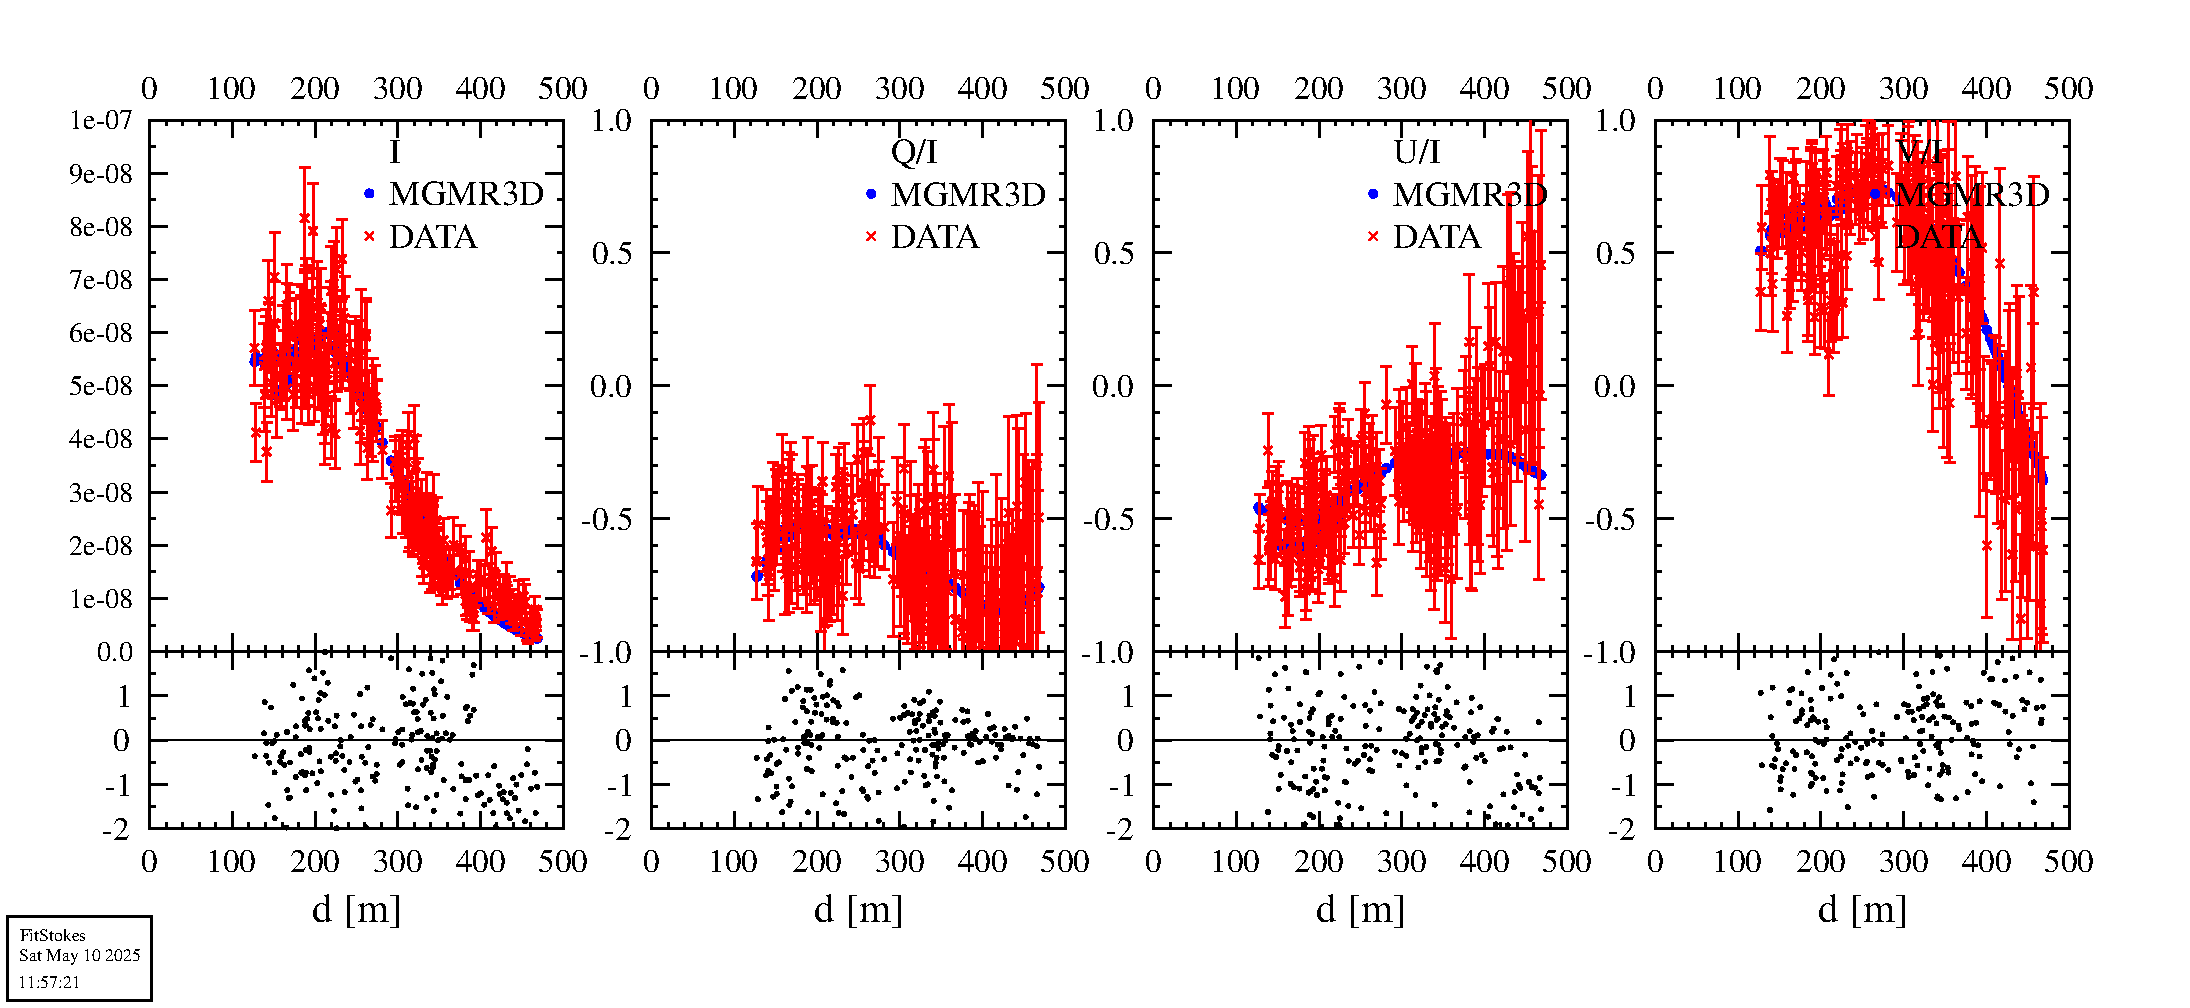
\includegraphics[width=0.99\textwidth]{runs/plot/FitStokes.pdf}
 \caption{The Stokes parameters (blue squares) are compared with those from a microscopic CoREAS~\cite{Hue13} calculation (red crosses). Also shown are the relative deviations (times 10) for the intensities and the differences (times 10) for the other Stokes parameters.  \figlab{FitStokes}}
\end{figure}

\section{Compilation}

Batch files for running under Windows and Linux are part of the distribution. The command files for some of the common figures, using GLE (see \verb<http://www.gle-graphics.org/< for a free distribution) are also given. For completeness \verb<fftpack5.1d.f90< is also supplied.

The program used the double-precision version of FFTPACK (see \href{http://www.netlib.org/fftpack/}{http://www.netlib.org/fftpack/} and \href{http://people.sc.fsu.edu/~jburkardt/f_src/nl2sol/nl2sol.html}{NL2SOL} where the source of the latter is part of the package.

To compile NL2SOL from the source you may use
\\\verb< gfortran -c C:/OlafsUtil/LSQ/nl2sol.f90<
\\\verb< move nl2sol.o C:/OlafsUtil/LSQ/nl2sol.o<

To create the necessary FFTPACK library you can use something like
\\\verb< C:/OlafsUtil/NumLib/F-split/f90split   ../fftpack5.1d.f90<
\\\verb< gfortran -c *.f90<
\\\verb< ar rcs libFFTPack.a *.o<
\\\verb< copy libFFTPack.a C:/OlafsUtil/NumLib/bin/libFFTPack-d.a<

To compile MGMR3D you may run the supplied makefile using
\\\verb< make -f MGMR3D_fit-makefile.mak<

To run the program you can use
\\\verb<rums/MGMR3D_fit.bat<
\\from the distribution file.
All this works on my windows10 system. It should be easy to adapt this for LINUX.



\begin{thebibliography}{100}
  \setlength{\itemsep}{1pt}
  \setlength{\parskip}{0pt}
  \setlength{\parsep}{0pt}
  \small

\bibitem{Sch08} O. Scholten, K. Werner, and F. Rusydi, \Ttl{A Macroscopic Description of Coherent Geo-Magnetic Radiation from Cosmic Ray Air Showers} Astropart.\ Phys.\ \VYP[10.1016/j.astropartphys.2007.11.012]{29}{2008}{94}, \arXiv{0709.2872}.

\bibitem{MGMR3D} Olaf Scholten, Gia Trinh, Krijn D. de Vries, Brian M. Hare,
    \Ttl{Analytic calculation of radio emission from parameterized extensive air showers, a tool to extract shower parameters} \arXiv{1711.10164}.

\bibitem{Tri15} G. Trinh, O. Scholten, \etal, \Ttl{Influence of Atmospheric Electric Fields on the Radio Emission from Extensive Air Showers.} \PRD{93}{2016}{023003}, \arXiv{1511.03045}.

\bibitem{Hue13} T. Huege, M. Ludwig, C.W. James, AIP Conf. Proc. \VYP{1535}{2013}{128}; \arXiv{1301.2132}.


\end{thebibliography}

\end{document}
